\pagestyle{fancy}
\fancyhf{}
\renewcommand{\headrulewidth}{0pt}
\fancyfoot[C]{\leftmark}
\fancyhead[R]{\thepage}
\doublespacing
\chapter{Simulation techniques and model systems}\label{chap2}

\section{Introduction}
Computer simulations have evolved to be a powerful technique to explore the properties of a physical system, using appropriate mathematical description or modelling. Often, it allows us to complement experimental observations or even explore possibilities which are beyond experimental limits. There has been a significant increase in computer power in recent years, making possible the classical simulation of systems with up to a million atoms within reasonable computing hours. So, computer simulation has become an important tool to explore various statistical properties of materials to gain insights into their behaviour. Moreover, sometimes, designing and performing simulations is far cheaper and more convenient than experiments, and also provides access to relatively more information. 
    
The simulation technique to be used to solve a particular physical problem depends on many factors, viz. type of system, nature of the problem, available model, computational resources etc. Many of these techniques use the idea of statistical sampling to explore different parts of the phase space. The two most popular particle based classical simulation techniques for doing such phase space sampling are Monte Carlo (MC)\cite{binder2011glassy,metropolis1949monte,allen2017,frenkel2001understanding}, which has a stochastic approach, and Molecular Dynamics (MD) \cite{alder1957phase,alder1959studies,rahman1964correlations,binder2011glassy,allen2017,frenkel2001understanding}, which has a deterministic approach. In MC simulation, acceptance or rejection of a random change in configuration from one state to another is based on certain criteria defined by the thermodynamic constraints. The evolution of the system in such a scheme does not necessarily represent the true dynamics at a microscopic level. In contrast, MD involves the solving of Newton's equation of motion, given a well-defined interaction between constituents, to evolve the system from one state at time $t$ to another state at $t + \Delta t$, and this often mimics the microscopic dynamics.
    
MD provides a direct pathway to calculate the time evolution of dynamical quantities because of a very clear notion of time but such a notion is difficult in MC simulations. On top of this, since MD can mimic realistic microscopic processes, it is the correct method to use for simulating phenomena like shear flow. Hence, we make use of MD simulations to simulate heat transport, Couette flow, Poiseuille flow etc, and also study quiescent dynamics, in the coming chapters. Also, in one of our studies, we used MC to produce well-annealed samples of glasses following a recently developed technique. In the next two sections of this chapter, we will discuss the technicalities of MD and MC. Also, in the last section, two glass-forming models will be introduced which have been used to explore different phenomena in chapters 3, 4, 5 and 6. 

%%%%%%%%%%%%%%%%%%%%%%%%%%%%%%%%%%%%%%%
\section{Molecular dynamics simulations: equilibrium and non-equilibrium}
The primary requirement for an MD simulation is a well-defined interaction potential between the constituent particles whose dynamics will be explored to analyse the physical properties of the system under study. Once the force acting on each particle is known from the potential, then the task is to solve Newton's equation of motion for each particle, as discussed above. If appropriate initialization i.e., assigning of positions and velocities to all particles at $t = 0$, is done, then time can be discretised and Newton's equation can be solved using some appropriate integration algorithm at each time interval to advance the dynamics. Below in this section, we discuss the use of interaction potential which will be followed by the detailing of a popular integration scheme that we have used in our simulations. Then we discuss how periodic boundary conditions are used to remove the surface effects to match the properties of the bulk system. Also, we describe how a modified periodic boundary condition can be used to shear the system. Next, we outline a few numerical tricks which can be used to speed up the integrating procedure. This is followed by a discussion on constant temperature MD simulation. In the end, we briefly discuss the strategy to simulate a glass-forming liquid.

    %%%%%%%%%%%%%%%%%%%%%%%%%%%%%%%%%%%%%%%%%
    \subsection{Interaction potential}
    The interaction between the particles in a system can be modelled in terms of potential. We can consider the interaction to be pairwise, in the simplest case. For such potential, the inter-particle force is calculated using the derivative of the potential with respect to inter-particle separation. More details on the type of interaction potentials that we have used in our study can be found in section-\ref{model}.
    
    %%%%%%%%%%%%%%%%%%%%%%%%%%%%%%%%%%%%%%%%%%
    \subsection{Integrating the equation of motion}
    
    For a $N$ particle system, $N$ number of Newton's equations can be written with $i \in \{1, 2, ..., N\}$:
    \begin{equation}
        m_i \ddot{\bf r}_i = \sum_{j(\neq i)} {\bf F}_{ij}.
    \end{equation}
    Here $m_i$ is the mass of $i$th particle at position ${\bf r}_i$ and ${\bf F}_{ij}$ is force between particle $i$ and $j$. The numerical solution of the above equations can be obtained by employing an integrator, to obtain positions and velocities. An appropriate integrator should be easily implementable, symplectic and satisfying time-reversal symmetry. Symplecticness of the integrator guarantees energy conservation and volume preservation in phase space \cite{bond1999nose}. One such integrator is {\em velocity-Verlet} \cite{verlet1967computer} algorithm which has an error of the order of $\delta t^4$ ($\delta t$ is time step). In this scheme, the new positions and velocities at time $t + \delta t$ can be obtained by
    \begin{equation}
        \textbf{r}_i(t+\delta t) = \textbf{r}_i(t) + \textbf{v}_i(t)\delta t + \frac{\textbf{F}_i(t)}{2m_i}\delta t^2,
    \end{equation}
    \begin{equation}
        \textbf{v}_i(t+\delta t) = \textbf{v}_i(t) + \frac{\delta t}{2m_i} [\textbf{F}_i(t+\delta t) + \textbf{F}_i(t)].
    \end{equation}

    In this thesis, our focus is on simulating non-equilibrium phenomena. In those circumstances,  the equations of motion need to be modified appropriately depending upon protocol. For example, to simulate Poiseuille flow \cite{evansMorrissBook,todd1995,todd1995pressure}, an external force is introduced into the equation of motion (see chapter-\ref{chap5} for more details). Also, for simulating Couette shear flow, {\em SLLOD} equations of motion \cite{evans1984nonlinear,evansMorrissBook} are often utilised, where some additional terms are introduced to the equations of motion such that a linear velocity profile is enforced. Further, in the case of the temperature gradient, non-equilibrium simulation can be achieved by local thermostatting, where we have local Langevin thermostats (see discussion below) which modify local equations of motion; see  Chapter-\ref{chap3} and \ref{chap4}. 
    
    %We have used Langevin thermostat (to be discussed below) to perform local thermostatting in  to impose a temperature gradient where the equations of motion are modified.
    
    For many simulations performed in different chapters of this thesis, we have used LAMMPS (Large-scale Atomic/Molecular Massively Parallel Simulator) \cite{lammps}, a very popular open-source MD simulator, to integrate the equations of motion in MD simulation. The major part of the source code in LAMMPS is written in C++ and most of the widely used potentials are available within LAMMPS, which is why this is used by a very large community all over the world. LAMMPS can be run very efficiently over a parallel architecture of computers, to handle a system of up to a few million atoms. The concept of domain decomposition is used in LAMMPS by dividing the simulation box into many sub-cells, to assign each sub-cell or domain to each processor.
    
    %%%%%%%%%%%%%%%%%%%%%%%%%%%%%%%%%%%%%%%%%
    \subsection{Boundary condition}
    In general, we are interested in situations where the system is infinite-sized, i.e. independent of any surface or wall/confinement effect. But, the ability to handle system sizes in simulations is very much limited, in comparison with systems handled in experiments which have the number of particles of the order of Avogadro's number ($\sim 10^{23}$). So, to simulate a typical bulk system with properties similar to real-life systems, periodic boundary conditions (PBC) are used, where the simulation box is replicated in all possible independent spatial dimensions \cite{allen2017,frenkel2001understanding}. Whenever a particle leaves the simulation box, it is entered again from the opposite side. In this way, it is possible to mimic a situation where the system can be treated as pseudo-infinite.
    
    \begin{figure}[hbt!]
	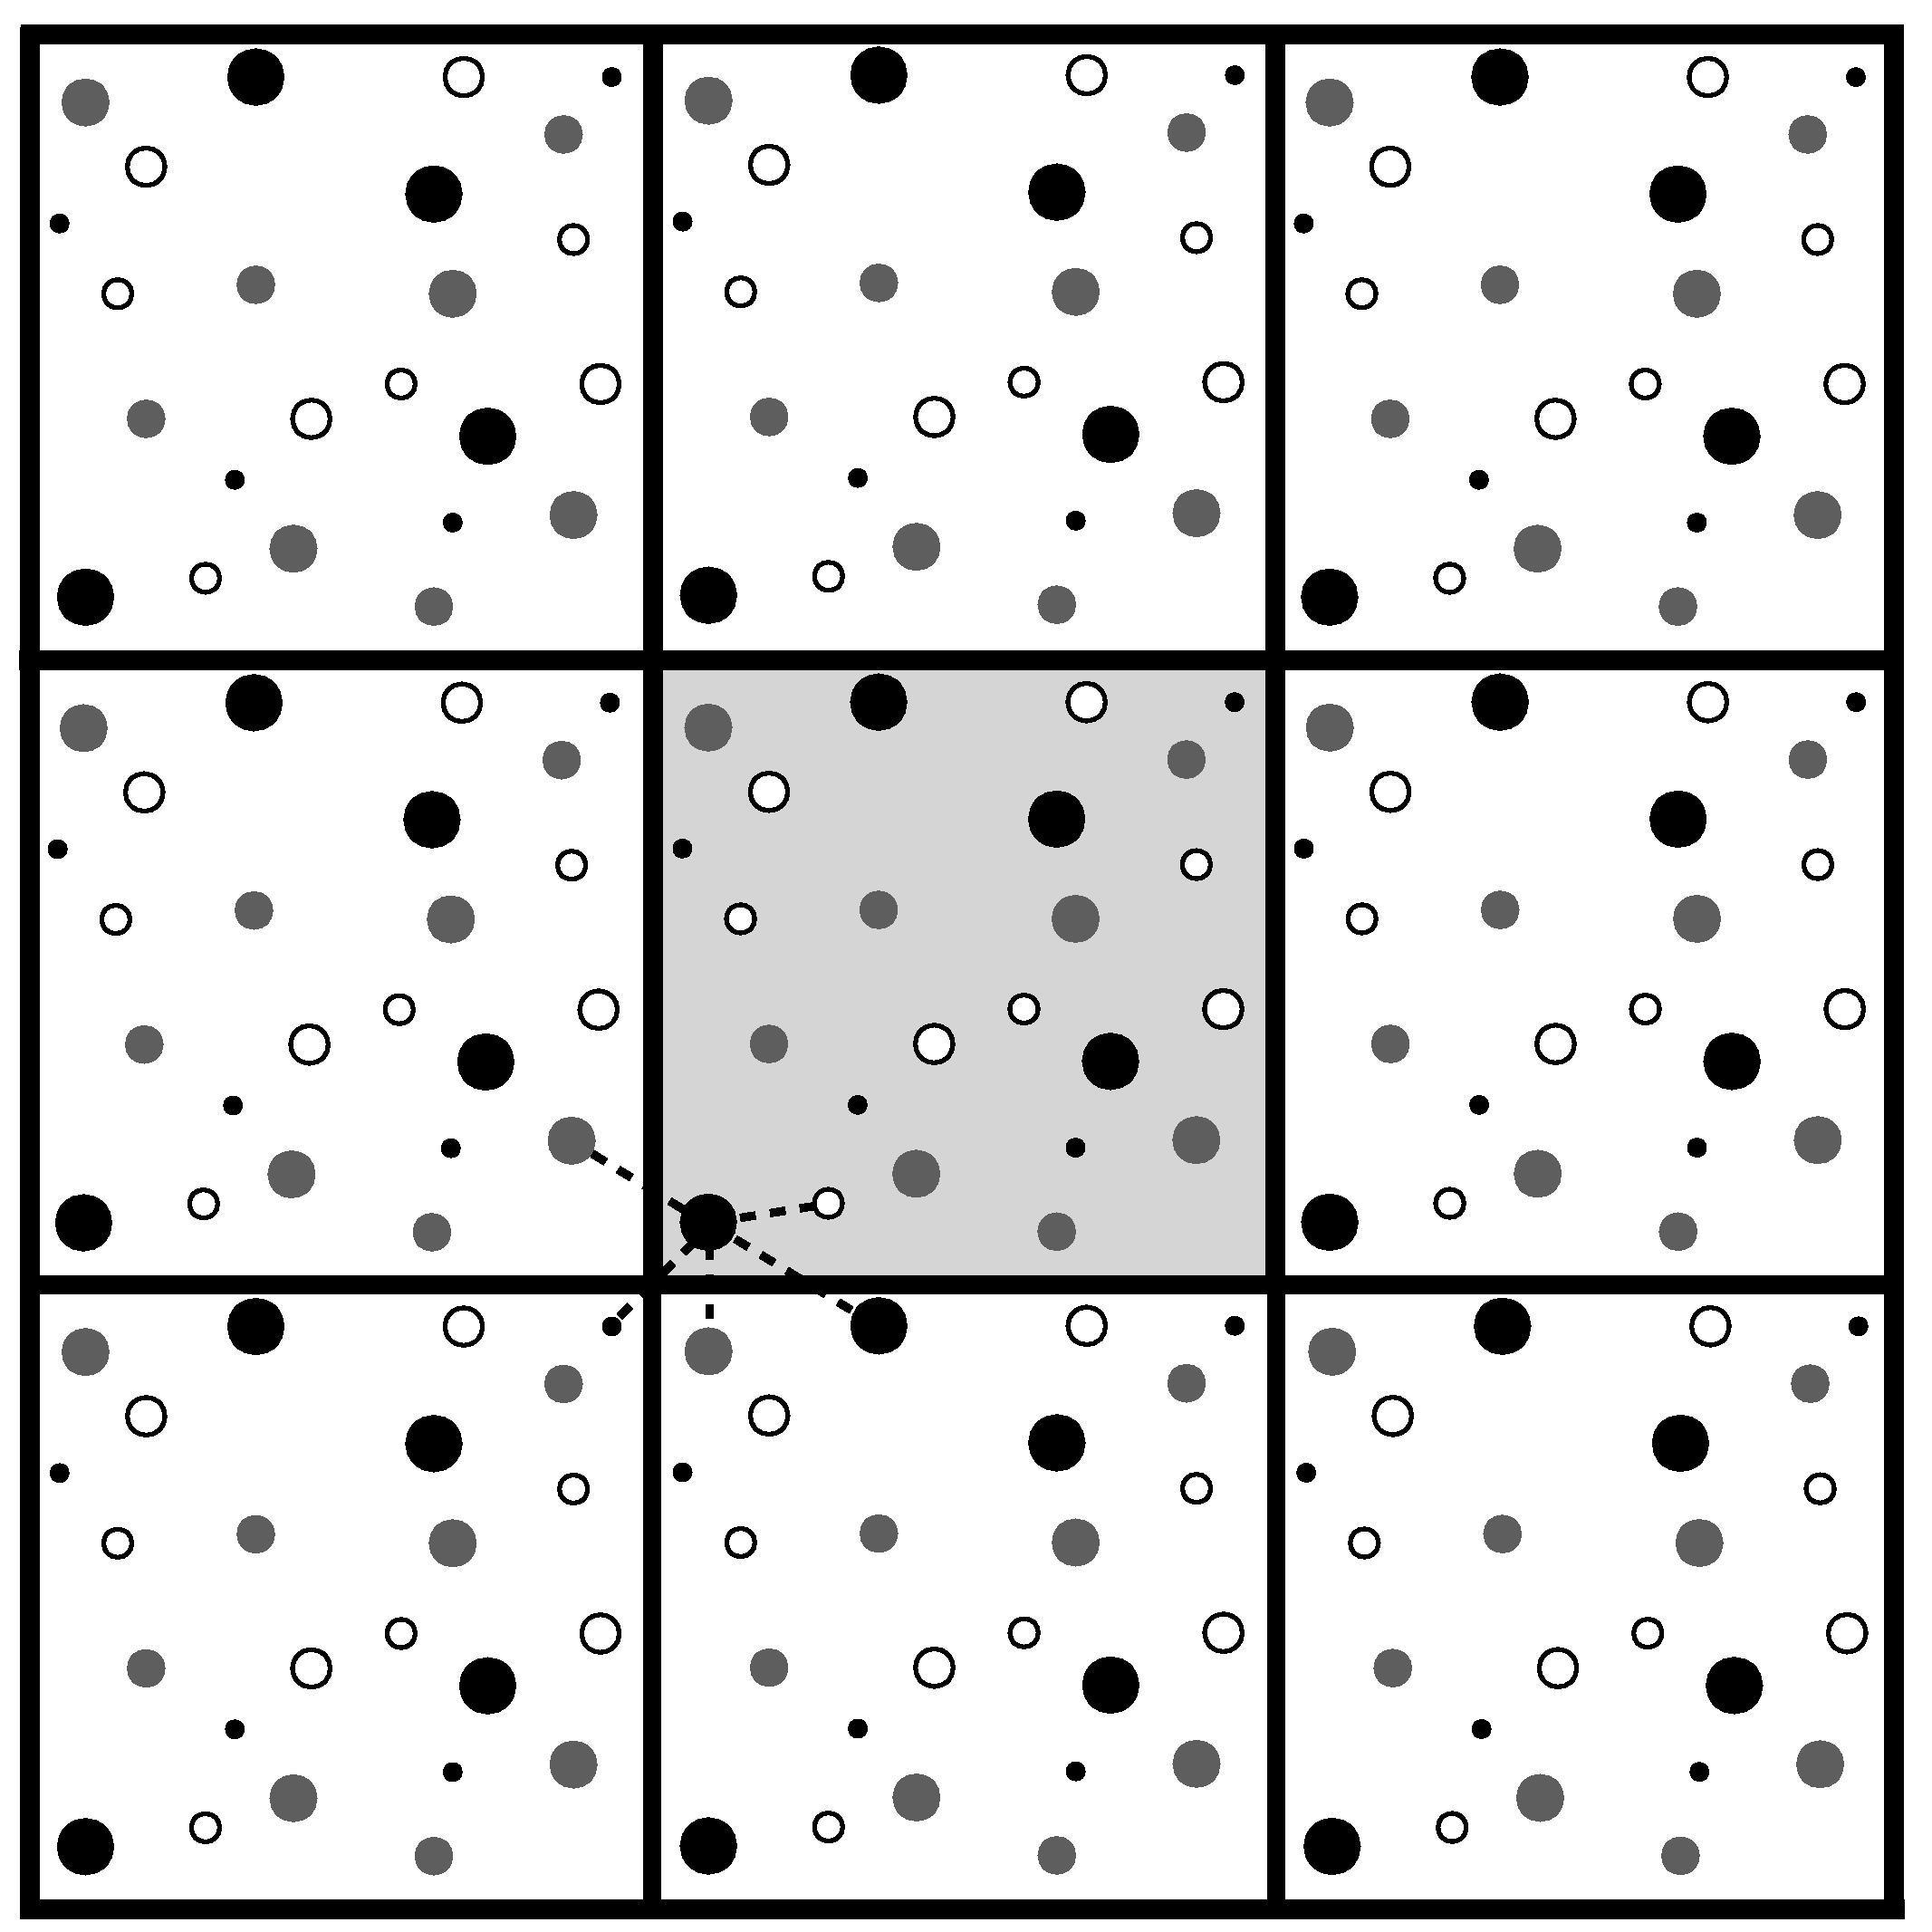
\includegraphics[width=12cm]{figs/pbc.pdf}
	\centering
	\caption[{\em Schematic representing the periodic boundary conditions}]{Schematic representing the periodic boundary conditions for a two-dimensional system.\label{pbc}}
    \end{figure}
    
    In a PBC setup, each particle can interact with all other particles in the same box and also in replica boxes, including the interaction with the images of the particle itself in replicas, resulting in an infinite series summation of interactions. To simplify the calculation, for a system with short-range interactions only, a scheme called {\em minimum image convention} is considered. In this scheme, we consider the interaction of a particle with any other particle or its image such that the inter-particle distance is minimum. This convention is effective only if the cutoff of the interaction $r_c$ is less than half of the box length.
    
    {\bf \em Boundary conditions for a deformed system:} Shear flow experiments are generally carried out by performing relative displacement of confining walls where the friction due to the walls causes the flow of the liquid. However, simulating shear flow in MD simulation, for a realistic system, requires the above discussed PBC. But, it has to be suitably modified. In principle, it is possible to simulate shear flow by moving the confining walls (Couette flow setup) but this will introduce confinement effects into the system. Since we want to simulate bulk system properties, a modified PBC called {\em Lees-Edwards boundary condition} \cite{allen2017} is utilised. 
    
    \begin{figure}[hbt!]
	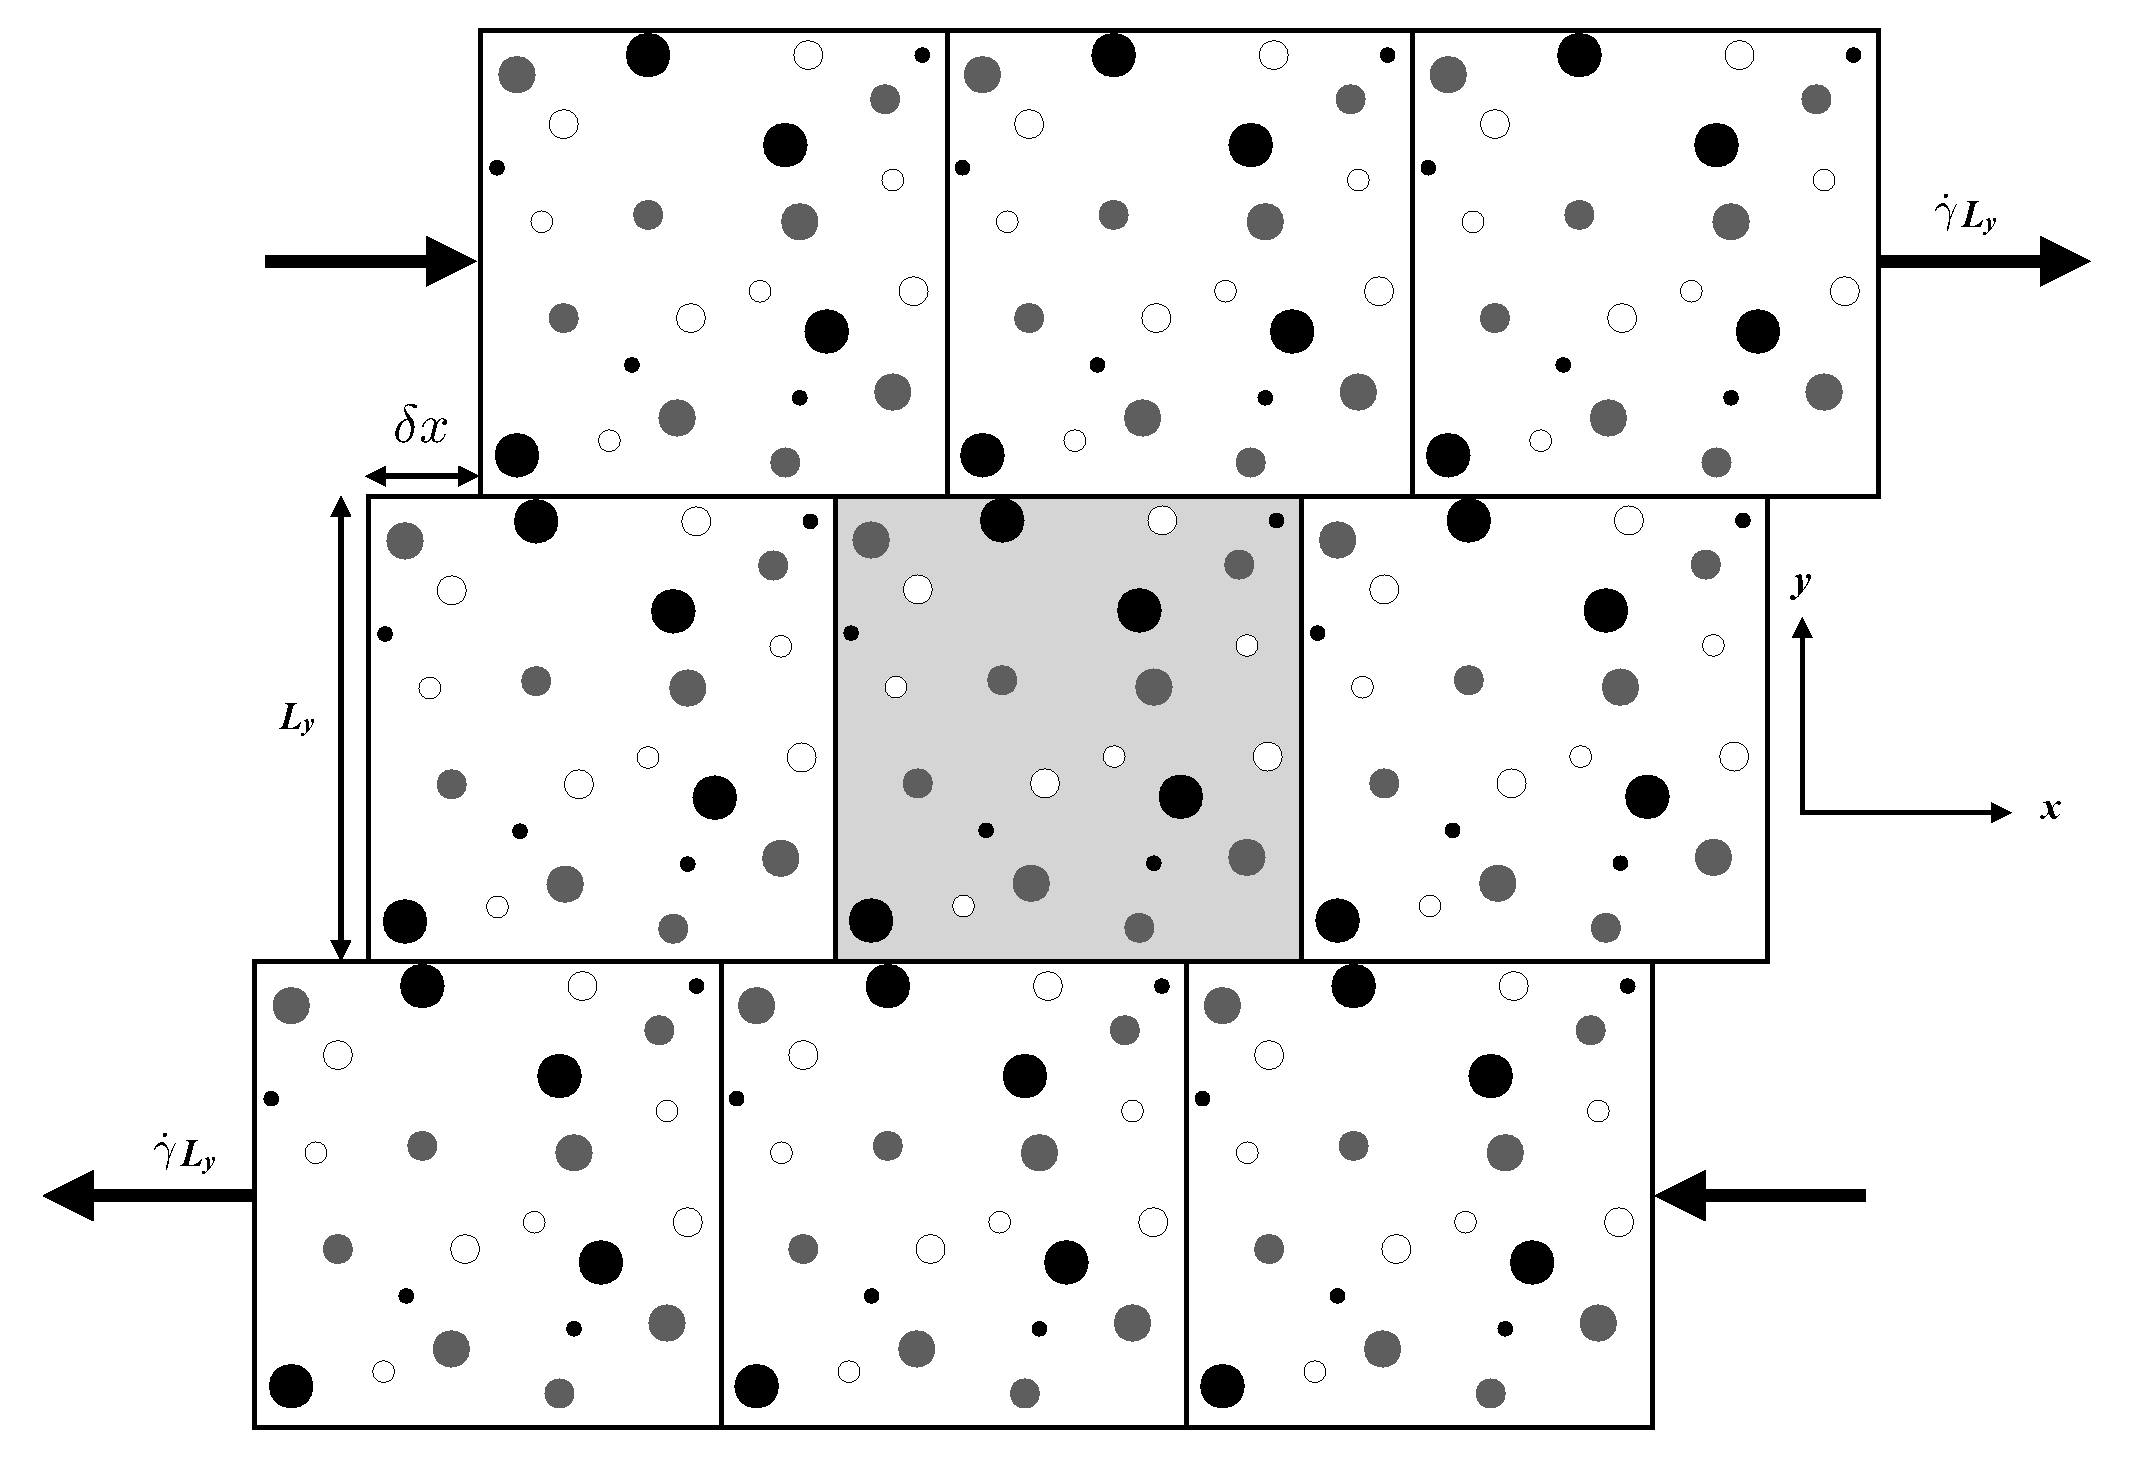
\includegraphics[width=14cm]{figs/LEpbc.pdf}
	\centering
	\caption[{\em Schematic representing the Lees-Edwards boundary condition}]{Schematic representing the Lees-Edwards boundary condition for a two-dimensional system.\label{LEpbc}}
    \end{figure}
    
    In this scheme to simulate a fixed shear rate simulation where $xy$-plane is sheared with shear-rate $\dot{\gamma}$ in the $x$-direction, the layer of periodic images just above the simulation box in the gradient direction move with velocity $\dot{\gamma}L_y$, in the direction of shear and the layer below move in the opposite direction (see Fig.~\ref{LEpbc}), while the layer containing the simulation box doesn't move.
     
    The displacement of the upper or lower layers, with respect to the central layer,  is made in the direction of shear or opposite to it in the following way: $\delta x = \dot{\gamma} t L_y$ (t is the time elapsed since the start of shear). Now, the crossing of the boundary in the flow and vorticity direction is done based on the periodic boundary conditions but in the gradient direction, the following steps are followed:
    \begin{itemize}
        \item If boundary is crossed at $y = L_y$ ($y = 0$), $L_y$ is subtracted (added).
        \item $\delta x$ is subtracted (added) to the $x$-coordinate of each particle.
        \item $\dot{\gamma}L_y$ is subtracted (added) to the $x$-component of velocity of each particle.
    \end{itemize}
    Also, the minimum image convention is modified for the direction of flow i.e., $x$. For a pair of particles $i$ and $j$, to calculate the inter-particle separation of $j$ from $i$, the following steps are considered:
    
    \begin{itemize}
        \item If the $j$th particle is in the primary simulation box is closest in the $y$-direction then the usual minimum image convention is applied in $x$-direction
        \item If the image of $j$th particle in the upper (lower) layer is closest in the $y$-direction then $\delta x$ is subtracted (added) to the inter-particle separation in the $x$-direction before applying the usual minimum image convention.
    \end{itemize}
    
    %%%%%%%%%%%%%%%%%%%%%%%%%%%%%%%%%%%%%%%%%%
    \subsection{Neighbour list and cell list}
    In an MD simulation, the most time consuming step is the force calculation using the chosen pair-potential, which involves the inter-particle distance calculation. For a $N$ particle system, the number of possible pairs is $N(N-1)/2$, which means, the force calculation has a computational complexity of the order of $N^2$. One way to reduce the computational cost is to use the concept of the neighbour list. When this technique is used, then a list is constructed for all possible pairs that are in the neighbourhood of each other, based on a cutoff ($r_c + {\rm skin}$) slightly larger than the cutoff for pair-potential \cite{allen2017,frenkel2001understanding,grest1989vectorized}.  This extra width added to the pair-potential cutoff $r_c$ is called skin width. Further, this list can be used for inter-particle separation calculation to know the force acting on each pair. The construction of the neighbour list has the computational complexity of $N^2$ but this way of calculating the force pairs using the neighbour list has the computational complexity of $N$. The advantage that we get in this method of force calculation is that the same list can be retained up to a few time steps i.e., the expensive inter-particle separation calculation is not done at each time step; rather, the neighbour list is used for inter-particle separation calculation. For the number of time steps, the neighbour list can be retained -- it depends on the state of the system, the nature of the pair potential, the length of the time step and the skin width. %The neighbour list can be full of half depending upon the type of calculation other than the force calculation. For {\em half neighbour list}, just all possible neighbour pairs for the given configurations, taking account the symmetry, are listed in a long one dimensional list but for {\em full neighbour list} all neighbours for a given particle are written together.
    
    Although implementing the neighbour list into an MD program makes it many orders faster, but it can be made even faster if the neighbour lists are constructed using cell lists i.e., it will have a complexity less than the $N^2$. The cell list keeps a track of all the particles belonging to different small cells obtained by dividing the simulation box. To create a cell list, all the particles are traversed and depending on their position, different cells are assigned. This process has the complexity of order $N$. After constructing the cell list, different cells are traversed to calculate the neighbour list. It should be noted that while constructing the cell list, the dimension of the cell should not be less than the $(r_c+skin)$. Also, during traversing the cell, only $14$ out of $27$ in $3-D$ and $5$ out of $9$ in $2-D$ should be considered for inter-particle distance calculation, because of the symmetry. 
    
    %%%%%%%%%%%%%%%%%%%%%%%%%%%%%%%%%%%%%%%%%%%%%%%%%%
    \subsection{Simulation at fixed temperature: thermostats}\label{thermostat}
    If Newton's equations of motion are integrated for a given pair-potential, the system by definition is in the micro-canonical ensemble. Therefore, the total energy of the system is fixed, and the temperature of the system fluctuates. But, on many occasions, we intend to simulate the system at a particular temperature, i.e. sample states within the canonical ensemble. For such purpose, we need to use a thermostat which modifies the velocity or sometimes the equation of motion, to have control over the temperature of the system \cite{allen2017,frenkel2001understanding}. Thermostats like velocity rescaling, Berendsen thermostat, Andersen thermostat etc. modify the velocity of the system at each time step or an interval of time steps to control the temperature. Such thermostats are very easy to implement and have very little computational cost but do not adhere to the canonical state of the system. On the other hand, thermostats like Langevin thermostat, Nose-Hoover thermostat etc. modifies the equation of motion to control the temperature of the system and are very much physical in many respects. Langevin thermostat is a very popular thermostat when dealing with colloids and has a closer resemblance with experiments. Nose-Hoover thermostat is very popular because it produces true configurations of the canonical ensemble. So, whenever a calculation is to be done with a system under a constant temperature environment,  Nose-Hoover thermostat is often preferred over other thermostats.
    
    {\bf \em Langevin thermostat:} As indicated above, Langevin thermostat \cite{frenkel2001understanding,allen2017} is implemented by modifying the equations of motion. A dissipative force ${\bf F}^{\rm D}_i = - \gamma v_i $, depending on the velocity of the particle and friction constant $\gamma$, and a random force ${\bf F}^{\rm R}_i$ act on each particle, other than the usual conservative force ${\bf F}^{\rm C}$ acting on the particle. So, the total force acting on $i$th particle is modified to the following:
    
    \begin{equation}
        {\bf F}_i = \sum_{j(\neq i)} {\bf F}^{\rm C}_{ij} + {\bf F}^{\rm D}_{i} + {\bf F}^{\rm R}_{i} .
    \end{equation}
    
    The random force is usually implemented in the form of white noise with zero mean and a variance given by,
    
    \begin{equation}
        \langle {\bf F}^{\rm R}_{i} (t)  {\bf F}^{\rm R}_{j} (t') \rangle = \Gamma^2 \delta_{ij}\delta(t-t').
    \end{equation}
    
    Here, $\Gamma$ is related with the temperature $T$ of the system and the dissipation constant $\gamma$ via the {\em fluctuation-dissipation} relation \cite{van1992stochastic}: $\Gamma = \sqrt{6k_BT\gamma}$. 
    
    {\bf \em Dissipative Particle Dynamics {\rm (DPD)} thermostat:} This thermostat \cite{dpd} is Galilean invariant and conserves the momentum locally, unlike the other thermostats discussed above, and also able to reproduce the correct hydrodynamic behaviour at sufficiently large length and time scales. Hence, the DPD thermostat is widely used to simulate rheological systems. In such systems, flow properties can be affected if a general thermostat is directly applied to particle velocities\footnote{Some other alternative approaches have been adopted but they generally affect the transient behaviour: (a) thermostat is applied after subtracting the local flow velocity and then flow velocity is added back. (b) thermostatting is done in other directions perpendicular to flow.}.
    
    The form of this thermostat is very similar to Langevin thermostat: a dissipative force ${\bf F}^{\rm D}$ depending on relative separation \& relative velocity and a pairwise random force ${\bf F}^{\rm R}$ is considered with the conservative pair interaction ${\bf F}^{\rm C}$ such that the total force ${\bf F}_i$ on a particle $i$ is given by
    
    \begin{equation}
        {\bf F}_i = \sum_{j(\neq i)} [ {\bf F}^{\rm C}_{ij} + {\bf F}^{\rm D}_{ij} + {\bf F}^{\rm R}_{ij}  ].
    \end{equation}
    
    Here, all forces act between a pair of particles, hence conserving momentum locally. The dissipative force depending on the relative separation (${\bf r}_{ij} = {\bf r}_i - {\bf r}_j$) and relative velocity (${\bf v}_{ij} = {\bf v}_i - {\bf v}_j$), has the following form:
    
    \begin{equation}
        {\bf F}^{\rm D}_{ij} = -\gamma \omega^{\rm D}(r_{ij}) [{\bf \hat{r}} _{ij}\cdot{\bf v}_{ij}] {\bf \hat{r}} _{ij},
    \end{equation}
    
    with $\gamma$ as the damping parameter and $\omega^{\rm D}$ as the weight function controlling the spatial variation of the damping term. The random force depending on the relative separation (${\bf r}_{ij}$), has the following form:
    
    \begin{equation}
    {\bf F}^{\rm D}_{ij} = \sigma \omega^{\rm R}(r_{ij}) \xi_{ij} {\bf \hat{r}} _{ij},
    \end{equation}
    
    with $\sigma$ as noise strength, $\omega^{\rm R}$ as weight function controlling spatial variation of strength and $\xi_{ij} = \xi_{ji}$ are random numbers independently sampled for different pair of particles and at different times, from Gaussian distribution with zero mean and unit variance. All parameters are not independent here, to satisfy the fluctuation-dissipation theorem:
    
    \begin{equation}
        \omega^{\rm D}(r_{ij}) = [\omega^{\rm R}(r_{ij})]^2,
        \sigma = \sqrt{2k_BT\gamma}.
    \end{equation}

    It should be noted that similar to the case of pair interaction, a cutoff $r_c^{\rm DPD}$ is used here to limit the applicability of the thermostat. The choice of weight function is very arbitrary and seems to limit only computational efficiency and temperature stability. In our study, we have considered the following form for weight function\footnote{this is the default weight function in LAMMPS}:
    
    \begin{equation}
        \omega^{\rm D}(r_{ij}) = 1 - \frac{r_{ij}}{r_c^{\rm DPD}}.
    \end{equation}
    
    Therefore, to apply the DPD thermostat, we have to specify three independent parameters: temperature $T$, damping parameter $\gamma$ and the cutoff $r_c^{\rm DPD}$.
    
    \subsection{Simulating glass-forming liquids}
    
    The general strategy to simulate a glass-forming liquid using MD \cite{binder2011glassy,hansen2013} is to start with an appropriate model system and equilibrate it \footnote{To ensure equilibration of a system, the best thing is to monitor different thermodynamics quantities like temperature, energy etc., whether they reach a fixed value with reasonably small fluctuation. Another rigorous way could be to measure quantities like MSD, Self-intermediate scattering function etc. with different time origins, to ensure time translational invariance} at its high temperature liquid state far above the melting temperature of the model. To obtain a supercooled state, the well-equilibrated high temperature liquid is quenched to supercooled regime and constant temperature dynamics are run for at least few hundred times the relaxation time at that temperature. Hence, to prepare a well-equilibrated supercooled liquid configuration at a temperature very close to $T_{\rm MCT}$, the equilibration run could be very long. Glassy states very close to glass transition temperature are prepared either by cooling the high temperature state at some particular rate or by direct quenching the high temperature state to the glassy state. Since, most of the time, it is not possible to obtain properly annealed glasses at very low temperatures, the obtained glassy configuration is protocol dependent. Hence, it is customary to mention the preparation protocol whenever glassy samples are generated. In the next section, a simulation technique has been discussed which has been successful in preparing well-annealed glassy samples at very low temperatures for some specific type of polydisperse model system.
    
\section{Swap Monte Carlo simulation}\label{swap}
There is a drastic increase in structural relaxation timescales as we move closer to the glass transition. Because the timescales accessible in conventional simulations is very limited, it has not been possible to equilibrate the glass-forming liquid very close to the glass transition. But Swap Monte Carlo (SMC) Algorithm \cite{ninarello2017models} uses the idea of exchange of diameters in combination with a spatial displacement of particles, to allow faster structural relaxation. This scheme uses the Metropolis criteria to perform the moves, which uses the Boltzmann weight satisfying detailed balance. SMC has been applied to glass-forming models with continuous size polydispersity, and it has been very successful in equilibrating samples at very low temperatures below $T_{\rm MCT}$ in reasonable computational time.
    
{\bf \em Hybrid SMC MC-MD:} A hybrid combination of SMC and MD \cite{berthier2019,ozawa2018random} can be implemented, where the diameter exchange of particles is performed at an interval of few MD time steps. In our implementation, after each $t_{\rm MD}$ time, SMC moves are attempted which is equal to the number of participating particles. During each SMC move, two particles are randomly chosen and their diameters are exchanged. If $\Delta E$ be the change in energy of the system during this process, then based on the Metropolis criterion, the exchange of diameters is accepted or rejected: accepted with probability min$\{1, {\rm exp}(-\Delta E/ (k_B T))\}$ otherwise rejected. Here $T$ is the temperature at which equilibration is done.
    
{\bf \em Numerical setup:} Efficient calculation of energy difference $\Delta E$ is crucial for SMC. It should be noted that during one exchange of pair diameters, only the pair interactions associated with the two particles participating in the exchange process, are affected. So, it is sufficient to calculate the pair energy of two particles with their neighbours within the cutoff, before (initial energy) and after (final energy) the  exchange of diameters. For this calculation, the full Verlet list should be used, where all neighbours (based on pair potential cutoff) for each particle are listed. Also, if we want to use the same Verlet list for the whole sequence of SMC moves invoked after each $t_{\rm MD}$ time, then the Verlet list should be built considering the polydispersity i.e., the cutoff used to build the Verlet list should be valid for the two particles with largest diameters. Note that after finishing all SMC attempts, force calculation should be updated before restarting the MD steps.
    
\section{Model glass-forming liquids}\label{model}
In this thesis, we have used two different models of glass-forming liquids: Kob-Andersen binary Lennard-Jones mixture and purely repulsive binary mixture with large size bidispersity. The first model has been used in studying thermal response and Poiseuille flow of glassy liquids, while the second model is very special, and has been used to study the rheology of materials with the presence of particles of very different sizes. We discuss the details of these two models below, which will be referred to in the coming chapters. But, at first, let's understand the generic nature of pair potential.

The generic potential should be repulsive for small separations of particles and attractive for large separations. The repulsive part of the potential at small separations is crucial in determining the structural properties of the liquid as well as solidification, while the attractive part has consequences for liquid-gas transitions. In many cases, only a short-range repulsive part is sufficient to simulate different properties of the system. In our work, we have mainly used the {Lennard-Jones model potential} to perform different studies.
    
    {\bf \em Lennard-Jones potential:} Insights from quantum mechanical calculations indicate that large distance inter-particle interaction should be of the form of $r^{-6}$ while short distance interaction can be approximated by the form ${\rm exp}(1/r)$. Due to computational advantages, the short-range interaction is approximated by inverse power law $r^{-n}$. Lennard-Jones form of potential considers $n=12$ for short range part:
    \begin{equation}
    V(r)= 4\epsilon \Bigg[\Big(\frac{\sigma}{r}   \Big)^{12} -\Big(\frac{\sigma}{r}   \Big)^6  \Bigg].
    \end{equation}
    Here the parameter $\sigma$ is the separation of the particles where $V(r)=0$ and $\epsilon$ is the depth of the potential well at the minimum in $V(r)$.
    
    Most of the time, the pair-potential vanishes quickly as the inter-particle distance increases. Example of such a short-ranged potential is Lennard-Jones potential, Yukawa potential, Harmonic potential, DLVO potential etc. In this case, it is useful to cut the potential at an appropriate distance (say at $r_c$), not only to simplify the numerical calculation but also to increase the efficiency of potential energy or force calculation. However, there are many model interaction potentials which are not short-ranged, for example- Coulombic interaction, gravitational interaction etc. Then, special techniques (like Ewald sum) are employed. Discussion of special techniques related to the long-range potential is beyond the scope of this chapter. When the cutoff is introduced to the interaction potential, it is advisable to consider a mathematical construction beyond the cutoff distance, which ensures the continuity of potential and its higher-order derivatives at the cutoff. Such smoothing constructions are crucial for many numerical calculations.

{\bf \em Kob-Andersen binary Lennard-Jones mixture:} This is a well-studied glass-forming model \cite{Kob94} in the form of Lennard-Jones potential, whose various properties have been well characterized in different studies. This model binary mixture has a 80:20 composition of the two species A and B respectively. Within the mixture, the interaction at a distance $r$ between two particles labelled $\alpha$ and $\beta$ has the following form:

\begin{eqnarray}
\label{LJ1}
\textrm{V}_{\alpha\beta}(r) &=&  u_{\alpha\beta}(r)-u_{\alpha\beta}(R_{c})-\left(r-R_{c}\right)\left. \frac{du_{\alpha\beta}}{dr}\right|_{r=R_{c}},\nonumber\\
u_{\alpha\beta}(r) &=& 4\epsilon_{\alpha\beta}\left[\left(\sigma_{\alpha\beta}/r\right)^{12}- \left(\sigma_{\alpha\beta}/r\right)^{6}\right]\: ,
\end{eqnarray}

for $ r < R_{c} = 2.5\sigma_{\alpha \beta} $, with $\alpha, \beta = \textrm{A, B}$. $R_c$ is the cutoff distance at which the  potential $u_{\alpha\beta}(r)$ is truncated, and the form of $\textrm{V}_{\alpha\beta}(r)$ ensures its continuity at $r=R_c$. The different parameters take the following values \---\ for energy-scales:  $\epsilon_{\textrm{AA}} = 1.0$, $\epsilon_{\textrm{AB}} = 1.5\epsilon_{\textrm{AA}}$, $\epsilon_{\textrm{BB}} = 0.5\epsilon_{\textrm{AA}}$; and, for length-scales: $\sigma_{\textrm{AA}} = 1.0$, $\sigma_{\textrm{AB}} = 0.8\sigma_{\textrm{AA}}$, $\sigma_{\textrm{BB}} = 0.88\sigma_{\textrm{AA}}$. Each particle has the same mass $m=1$. We study this system at a number density of $\rho_0 = 1.2$, where this model system exhibits glassy behaviour upon decrease of temperature \cite{Kob94}.

All lengths are measured in the unit of $\sigma_{\rm AA}$, energy is expressed in the units of $\varepsilon_{\rm AA}$, the unit of time is $\sqrt{{m\sigma_{\rm AA}^{2}}/\epsilon_{\rm AA}}$ and that of stress is $\epsilon_{\rm AA}/ \sigma_{\rm AA}^{3}$. For this mixture,  the increase in relaxation timescales of the supercooled liquid with decreasing temperature can be fitted with mode coupling theory prediction, providing a mode-coupling critical temperature $T_{MCT} \approx 0.435$, below which conventional numerical simulations fail to obtain equilibrium dynamics. However, the putative glass transition temperature of the system, $T_{VFT} \approx 0.3$, is obtained by a Vogel-Fulcher-Tammam fit to the variation of relaxation timescale with temperature. 

{\bf \em Purely repulsive binary mixture with large size bidispersity:} The system that we study \cite{horbach2009} is a binary $50-50$ mixture of repulsive particles, where the diameter of the bigger particles (species A) is sampled from a uniform distribution, i.e.~$d_{\rm A} \in [0.85,1.15]$, while the diameter of the smaller particles (species B) is $d_{\rm B} = 0.35$ (see Fig.~\ref{fig6p1}). The average size ratio of A and B particles is $\langle d_{\rm A}\rangle/d_{\rm B} \approx 2.85$ where $\langle d_{\rm A}\rangle \approx 1$. A pair of particles $\{\alpha,\beta\}$ (with $\alpha = {\rm A, B}$ and $\beta = {\rm A, B}$), separated by a distance $r$, interacts via a Weeks-Chandler-Andersen (WCA) potential \cite{weeks1971}, i.e.~a Lennard-Jones potential that is cut off at its minimum and shifted to zero. To further smoothen the WCA potential, we also add a term that provides the continuity of its derivative. Thus, the potential is defined by 
%
\begin{eqnarray}
\textrm{V}_{\alpha\beta}(r) &=& u_{\alpha\beta}(r)-u_{\alpha\beta}(R_{c})-\left(r-R_{c}\right)\left.  \frac{du_{\alpha\beta}}{dr}\right|_{r=R_{c}},\nonumber\\
u_{\alpha\beta}(r) &=& 4\epsilon_{\alpha\beta}\left[\left(\sigma_{\alpha\beta}/r\right)^{12}- \left(\sigma_{\alpha\beta}/r\right)^{6}\right]\: ,
\end{eqnarray}
%
for $r<R_{c} = 2^{1/6} \sigma_{\alpha\beta}$, else $\textrm{V}_{\alpha\beta}(r) = 0$, with $\alpha, \beta$ as particle index. Here, $\sigma_{\alpha\beta} = (d_{\alpha}+d_{\beta})/2$ and $\epsilon_{\alpha\beta} = \epsilon = 1.0$ if both interacting particles are of the same type, else $\sigma_{\alpha\beta} = (1.00+0.35)/2$ and $\epsilon_{\alpha\beta} = 0.1$.  All particles have the same mass $m_{\rm A} = m_{\rm B} = m = 1$.  In the following, length, energy, and time are measured in units of $\langle d_{\rm A} \rangle$, $\epsilon$, and $\tau_{\rm WCA} = [m \langle d_{\rm A} \rangle ^2/\epsilon]^{1/2}$, respectively.

